\documentclass[10pt, landscape]{article}
\usepackage[scaled=0.92]{helvet}
\usepackage{calc}
\usepackage{multicol}
\usepackage[a4paper,margin=3mm,landscape]{geometry}
\usepackage{amsmath,amsthm,amsfonts,amssymb}
\usepackage{color,graphicx,overpic}
\usepackage{hyperref}
\usepackage{newtxtext} 
\usepackage{enumitem}
\usepackage[table]{xcolor}
\usepackage{mathtools}
\setlist{nosep}
% for including images
\graphicspath{ {./images/} }

\pdfinfo{
  /Title (CS2108.pdf)
  /Creator (TeX)
  /Producer (pdfTeX 1.40.0)
  /Author (Gavin Chiam)
  /Subject (CS2108)
/Keywords (CS2108, nus, cheatsheet, pdf)}

% Turn off header and footer
\pagestyle{empty}

% redefine section commands to use less space
\makeatletter
\renewcommand{\section}{\@startsection{section}{1}{0mm}%
  {-1ex plus -.5ex minus -.2ex}%
  {0.5ex plus .2ex}%x
{\normalfont\large\bfseries}}
\renewcommand{\subsection}{\@startsection{subsection}{2}{0mm}%
  {-1explus -.5ex minus -.2ex}%
  {0.5ex plus .2ex}%
{\normalfont\normalsize\bfseries}}
\renewcommand{\subsubsection}{\@startsection{subsubsection}{3}{0mm}%
  {-1ex plus -.5ex minus -.2ex}%
  {1ex plus .2ex}%
{\normalfont\small\bfseries}}%
\makeatother

\renewcommand{\familydefault}{\sfdefault}
\renewcommand\rmdefault{\sfdefault}
%  makes nested numbering (e.g. 1.1.1, 1.1.2, etc)
\renewcommand{\labelenumii}{\theenumii}
\renewcommand{\theenumii}{\theenumi.\arabic{enumii}.}
\renewcommand\labelitemii{•}
\renewcommand\labelitemiii{•}

\definecolor{mathblue}{cmyk}{1,.72,0,.38}
\everymath\expandafter{\the\everymath \color{mathblue}}

% Don't print section numbers
\setcounter{secnumdepth}{0}

\setlength{\parindent}{0pt}
\setlength{\parskip}{0pt plus 0.5ex}
%% adjust spacing for all itemize/enumerate
\setlength{\leftmargini}{0.4cm}
\setlength{\leftmarginii}{0.4cm}
\setlength{\leftmarginiii}{0.2cm}
\setlist[itemize,1]{leftmargin=2mm,labelindent=1mm,labelsep=1mm}
\setlist[itemize,2]{leftmargin=4mm,labelindent=1mm,labelsep=1mm}
\setlist[itemize,3]{leftmargin=4mm,labelindent=1mm,labelsep=1mm}

% adding my commands
\input{../commands/style-helpers.tex}
\makeatletter
\newcommand*{\xdashrightarrow}[2][]{%
  \mathrel{%
    \mathpalette{\da@xarrow{#1}{#2}{}\da@rightarrow{\,}{}}{}%
  }%
}
\newcommand*{\da@rightarrow}{\mathchar"0\hexnumber@\symAMSa 4B }
\newcommand*{\da@xarrow}[7]{%
  % #1: below
  % #2: above
  % #3: arrow left
  % #4: arrow right
  % #5: space left 
  % #6: space right
  % #7: math style 
  \sbox0{$\ifx#7\scriptstyle\scriptscriptstyle\else\scriptstyle\fi#5#1#6\m@th$}%
  \sbox2{$\ifx#7\scriptstyle\scriptscriptstyle\else\scriptstyle\fi#5#2#6\m@th$}%
  \sbox4{$#7\dabar@\m@th$}%
  \dimen@=\wd0 %
  \ifdim\wd2 >\dimen@
    \dimen@=\wd2 %   
  \fi
  \count@=2 %
  \def\da@bars{\dabar@\dabar@}%
  \@whiledim\count@\wd4<\dimen@\do{%
    \advance\count@\@ne
    \expandafter\def\expandafter\da@bars\expandafter{%
      \da@bars
      \dabar@ 
    }%
  }%  
  \mathrel{#3}%
  \mathrel{%   
    \mathop{\da@bars}\limits
    \ifx\\#1\\%
    \else
      _{\copy0}%
    \fi
    \ifx\\#2\\%
    \else
      ^{\copy2}%
    \fi
  }%   
  \mathrel{#4}%
}
\makeatother

% -----------------------------------------------------------------------

\begin{document}
\raggedright
\footnotesize
\begin{multicols*}{4}
  % multicol parameters
  \setlength{\columnseprule}{0.25pt}

  \begin{center}
    \fbox{%
      \parbox{0.8\linewidth}{\centering \textcolor{black}{
          {\Large\textbf{CS2108}}
        \\ \normalsize{AY24/25 SEM 2}}
        \\ {\footnotesize \textcolor{gray}{github/Gavino3o}}
      }%
    }
  \end{center}

  \section{\underline{Sinusoids}}

  \begin{itemize}
    \item Sinusoids are periodic functions that can be represented as a sum of sine and cosine functions. The general form of a sinusoid is:
    \begin{equation}
      y(t) = A \sin(\omega t + \phi) + B \cos(\omega t + \phi)
    \end{equation}
    where:
    \begin{itemize}
      \item $A$ is the amplitude
      \item $\omega$ is the angular frequency
      \item $\phi$ is the phase shift
      \item $B$ is the vertical shift
    \end{itemize}
    \item The angular frequency $\omega$ is related to the frequency $f$ and the period $T$ by:
    \begin{equation}
      \omega = 2\pi f = 2\pi \frac{1}{T}
    \end{equation}
    \item  Hence, the sinusoid can also be expressed in terms of frequency:
    \begin{equation}
      y(t) = A \sin(2\pi f t + \phi) + B \cos(2\pi f t + \phi)
    \end{equation}
  \end{itemize}

  \subsection{Discrete Time Sinusoids}
  \begin{itemize}
    \item Discrete time sinusoids are sampled versions of continuous time sinusoids. The general form is:
    \begin{equation}
      x[n] = \sum_{k=0}^{K-1} a_k \sin(2 \pi f_k t_n) + b_k \cos(2 \pi f_k t_n)
    \end{equation}
    where:
    \begin{itemize}
      \item $n$ is the discrete time index
      \item $k$ is the frequency index
      \item $t_n$ is the discrete time variable $n \Delta t$
      \item $f_k$ is the frequency of the $k$-th component $k \Delta f$
      \item $\Delta t$ is the sampling period
      \item $\Delta f$ is the frequency resolution
      \item $K$ is the total number of frequencies
    \end{itemize}
    The coefficients $a_k$ and $b_k$ define the amplitude and phase of each frequency component.
    \item The discrete time sinusoid can also be expressed in different forms:
    \begin{equation}
      \begin{aligned}
      x[n] & = \sum_{k=0}^{K-1} a_k \sin(2 \pi f_k t_n) + b_k \cos(2 \pi f_k t_n) \\ 
           & = \sum_{k=0}^{K-1} c_k \sin(2 \pi f_k t_n + \phi_k) \\ 
           & = \sum_{k=0}^{K-1} d_k \cos(2 \pi f_k t_n + \theta_k)
      \end{aligned}
    \end{equation}
    where:
    \begin{itemize}
      \item Second line is the same sinusoid a summation of shifted sine functions
      \item Third line is the same sinusoid as a summation of shifted cosine functions
      \item $c_k$ and $d_k$ are the coefficients for the sine and cosine forms
      \item $\phi_k$ and $\theta_k$ are the phase shifts for the sine and cosine forms
      \item The relationship between the coefficients is given by:
      \begin{equation}
        \begin{aligned}
          c_k & = \sqrt{a_k^2 + b_k^2} \\
          d_k & = \sqrt{a_k^2 + b_k^2} \\
          \phi_k & = \tan^{-1}\left(\frac{b_k}{a_k}\right) \\
          \theta_k & = \tan^{-1}\left(\frac{a_k}{b_k}\right)
        \end{aligned}
      \end{equation}
      \item If $a_k$ = $b_k$, the sinusoid is a combination of sine and cosine functions with equal amplitude and phase shift. Phase shift is 45 degrees.
      \item If $a_k$ = -$b_k$, the sinusoid is a combination of sine and cosine functions with equal amplitude and phase shift. Phase shift is 135 degrees.
      \item If $a_k$ = 0, phase shift is 90 degrees
      \item If $b_k$ = 0, phase shift is 0 degrees
    \end{itemize}
  \end{itemize}

  \subsection{Periodicity}

  \begin{itemize}
    \item Fundamental period is the smallest period of a sinusoid. The fundamental period is the time it takes for the sinusoid to complete one full cycle.
    \item The fundamental frequency is the reciprocal of the fundamental period:
    \begin{equation}
      f_0 = \frac{1}{T_0}
    \end{equation}
    \item The fundamental frequency is the lowest frequency of a sinusoid. It is the frequency at which the sinusoid oscillates.
    \item Sinusoids are periodic functions, meaning they repeat their values at regular intervals. 
    \item If we add sinoiuds with different frequencies, the resulting function is not periodic unless the frequencies are rationally related.
    \item Suppose we have a sinusoid with the equation:
     \begin{equation}
      y(t) = a_1 \sin(\omega_1 t + \phi_1) + a_2 \cos(\omega_2 t + \phi_2)
    \end{equation}
    \item To determine if the sinusoid is periodic, we need to check if the ratio of the \textbf{frequencies} is rational:
    \begin{equation}
      \frac{\omega_1}{\omega_2} = \frac{p}{q}
    \end{equation}
    where $p$ and $q$ are integers.
    \item To determine the \textbf{fundamental period} of the sinusoid, we need to find the least common multiple (LCM) of the periods of the individual sinusoids:
    \begin{equation}
      T = \text{lcm}(T_1, T_2)
    \end{equation}
    where $T_1$ and $T_2$ are the periods of the individual sinusoids. Calculate the period of each sinusoid using:
    \begin{equation}
      T_i = \frac{2\pi}{\omega_i}
    \end{equation}
    \item Hint: Let ratio of periods = $ \frac{T_1}{T_2} = \frac{q}{p}$, then $T = p T_1 = q T_2 $
    \item Suppose we have a sinusoid with the equation:
     \begin{equation}
      y(t) = a_1 \sin(2 \pi f_1 t + \phi_1) + a_2 \cos(2 \pi f_2 t + \phi_2)
    \end{equation}
    where $f_1$ and $f_2$ are integers
    \item To determine the \textbf{fundamental frequency} of the sinusoids, we need to find the greatest common divisor (GCD) of the frequencies of the individual sinusoids:
    \begin{equation}
      f = \text{gcd}(f_1, f_2)
    \end{equation}
    \item Then fundamental period is: $T = \frac{1}{f}$
    \item The above calculatiosn can be done with sinusoids of more than 2 frequencies as well.

  \end{itemize}


  
 \section{\underline{Fourier Series}}

  \subsection{Recap}
  \begin{itemize}
    \item \textbf{Orthogonal Basis Set} a set of functions that are orthogonal to each other. This means that the inner product of any two functions in the set is zero.
    \item Inner product of two functions $f(t)$ and $g(t)$ is defined as:
    \begin{equation}
      \langle f(t), g(t) \rangle = \int_{-\infty}^{\infty} f(t) g(t) dt
    \end{equation}
    \item Inner Product (continuous) = Dot Product (discrete)
    \item \textbf{Sine and cosine functions are orthogonal to each other}, no matter their frequencies. Inner/Dot product = \textbf{zero}.
    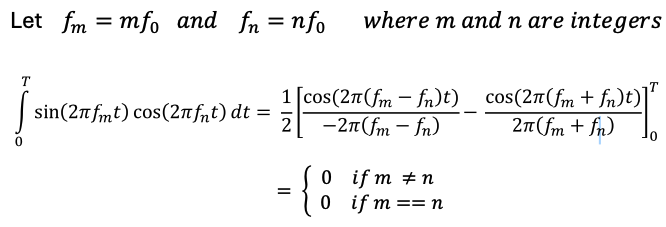
\includegraphics[width=0.95\linewidth]{sinecosineproduct.png} 
    \item \textbf{Sine waves of different frequencies} are orthogonal to each other.Inner/Dot product = \textbf{zero}.
    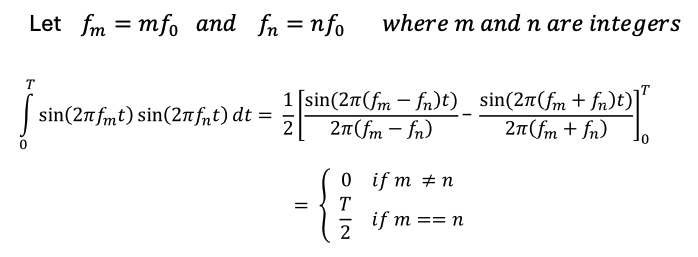
\includegraphics[width=0.95\linewidth]{sinesineproduct.png} 
    \item Similarly, \textbf{Cosine waves of different frequencies} are orthogonal to each other. Inner/Dot product = \textbf{zero}.
    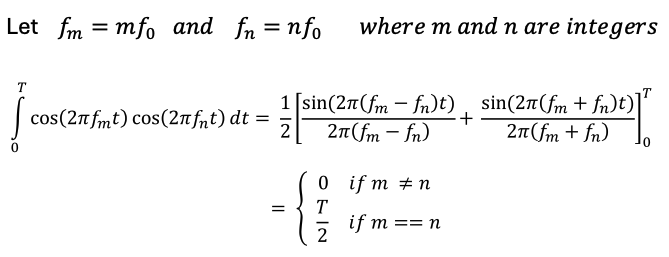
\includegraphics[width=0.95\linewidth]{cosinecosineproduct.png} 

    \item For sine and cosine with non-zero phase shifts:
    \begin{equation}
      \begin{aligned}
        & \sin(2 \pi f t + \phi) = sin(2 \pi f t) \cos(\phi) + \cos(2 \pi f t) \sin(\phi) \\
        & \cos(2 \pi f t + \phi) = cos(2 \pi f t) \cos(\phi) - \sin(2 \pi f t) \sin(\phi)
      \end{aligned}
    \end{equation}
    \item In other words, with a phase shift, a sine or cosine function that is phase shifted can be expressed as a weighted sum of sine and cosine functions. 
    \item So in general, the sum of sinusoidal signals, even with non-zero (but constant) phase, can be written as a linear combination of sine and cosine with zero phase.
    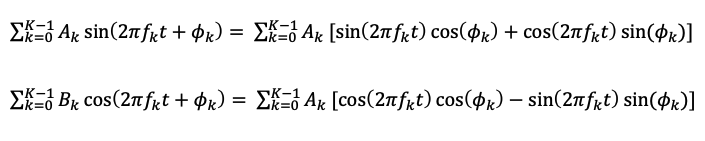
\includegraphics[width=0.95\linewidth]{phaseshiftconversion.png} 
  \end{itemize}


  \subsection{Fourier Series}

  \begin{itemize}
    \item Fourier series is a way to represent a periodic signal as a sum of sine and cosine functions. It is used to analyze periodic signals in the frequency domain.
    \begin{equation}
      y(t) = \sum_{m=0}^{M-1} (a_m \sin(2 \pi f_m t) + b_m \cos(2 \pi f_m t))
    \end{equation}
    \item How do we determine all of the $a_m$ and $b_m$: 
    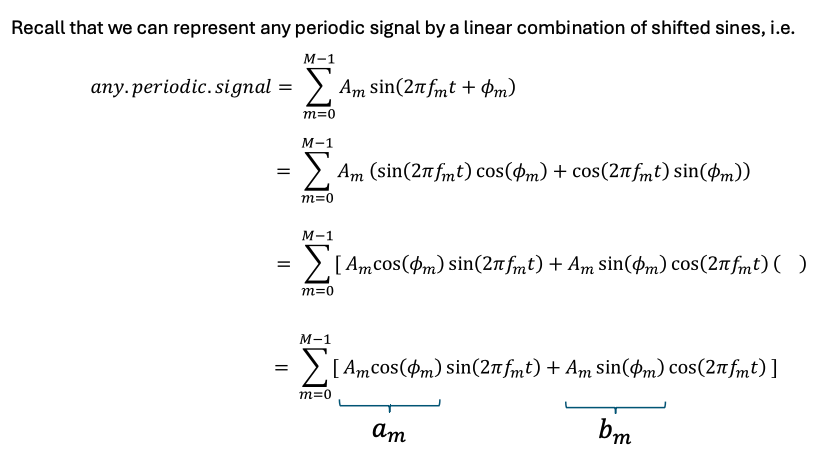
\includegraphics[width=0.95\linewidth]{ambm.png}
    \begin{equation}
      \begin{aligned}
        a_m & = A_m \cos(\phi_m) \\
        b_m & = A_m \sin(\phi_m)
      \end{aligned}
    \end{equation}
    \item The Fourier series coefficients $a_m$ and $b_m$ are calculated using the following formulas:
    \begin{equation}
      \begin{aligned}
        a_m & = \frac{2}{T} \int_{0}^{T} y(t) \sin(2 \pi f_m t) dt \\
        b_m & = \frac{2}{T} \int_{0}^{T} y(t) \cos(2 \pi f_m t) dt
      \end{aligned}
    \end{equation}
    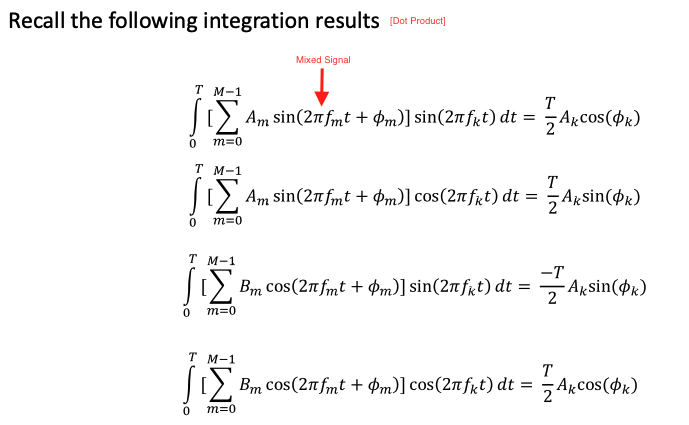
\includegraphics[width=0.95\linewidth]{signal_integration.png}
    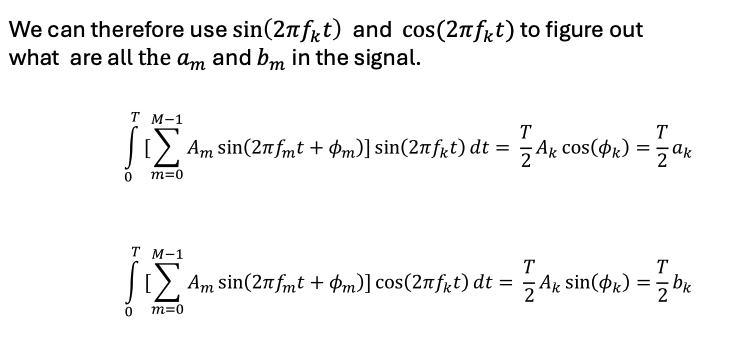
\includegraphics[width=0.95\linewidth]{finding_am_bm.png}
    \item The ratio of $b_k$ to $a_k$ gives the phase shift of the sinusoid:
    \begin{equation}
      \begin{aligned}
        & \ \frac{b_k}{a_k} = \frac{A_k \sin(\phi_k)}{A_k \cos(\phi_k)} = tan(\phi_k) \\
        & \phi_k = \tan^{-1}\left(\frac{b_k}{a_k}\right)
      \end{aligned}
    \end{equation}
    \item We can use complex numbers to represent the Fourier series:
    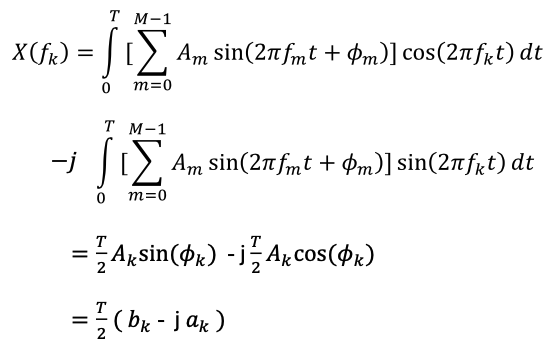
\includegraphics[width=0.95\linewidth]{fourier_series_complex.png}
    \item \textbf{Magnitude} = $|X_k| = \frac{T}{2}\sqrt{a_k^2 + b_k^2}$
    \item \textbf{Phase} = $\tan^{-1}\left(\frac{b_k}{a_k}\right)$
    \item We can also express the Fourier series in terms of \textbf{complex exponentials}, recall Eulers formula: $e^{j \theta} = \cos(\theta) + j \sin(\theta)$, then:
    \begin{equation}
      X(f_k) = \int_{0}^{T} [\sum_{m=0}^{M-1} A_m \sin(2 \pi f_m t + \phi_m] e^{-j 2 \pi f_k t} dt
    \end{equation}
    \item \textbf{Fourier series formula} (important):
    \begin{equation}
      X(f_k) = \int_{0}^{T} x(t) e^{-j 2 \pi f_k t} dt
    \end{equation}
  \end{itemize}

  \section{\underline{Fourier Transform}}
  \begin{itemize}
    \item Fourier transform is a way to represent a non-periodic signal as a sum of sine and cosine functions. It is used to analyze non-periodic signals in the frequency domain.
    \item \textbf{Intuition:} For non-periodic signals, we can think that its \textit{period is infinite}. Then the whole signal can be imagined as periodic with infinite period.
    \item Fourier series comparison:
    \begin{equation}
      X(f) = \int_{0}^{T} x(t) e^{-j 2 \pi f t} dt
    \end{equation}
    \item Fourier transform is defined as:
    \begin{equation}
      X(f) = \int_{-\infty}^{\infty} x(t) e^{-j 2 \pi f t} dt
    \end{equation}
    \item The inverse Fourier transform is defined as:
    \begin{equation}
      x(t) = \int_{-\infty}^{\infty} X(f) e^{j 2 \pi f t} df
    \end{equation}
    \item The Fourier transform can be used to analyze the frequency content of a signal. It can be used to determine the amplitude and phase of each frequency component in the signal.
    \item Fourier transform equation using radian frequency $\omega$:
    \begin{equation}
      X(\omega) = \int_{-\infty}^{\infty} x(t) e^{-j \omega t} dt
    \end{equation}
    \item The inverse Fourier transform using radian frequency $\omega$: 
    \begin{equation}
      x(t) = \frac{1}{2\pi} \int_{-\infty}^{\infty} X(\omega) e^{j \omega t} d\omega
    \end{equation}
    \item The Fourier transform can also be used to filter signals. By multiplying the Fourier transform of a signal by a filter function, we can remove or enhance certain frequency components in the signal.
    \end{itemize}

    \subsection{Discrete Fourier Transform (DFT)}

  \begin{itemize}
    \item \textbf{DFT} Formula:
    \begin{equation}
      X[k] = \sum_{n=0}^{N-1} x[n] e^{-j 2 \pi k \frac{n}{N}}
    \end{equation}
    \item \textbf{Inverse DFT} Formula:
    \begin{equation}
      x[n] = \frac{1}{N} \sum_{k=0}^{N-1} X[k] e^{j 2 \pi k \frac{n}{N}}
    \end{equation}
    where:
    \begin{itemize}
      \item $N$ is the number of samples
      \item $k$ is the frequency index (discretised frequencies)
      \item $n$ is the time index
      \item $x[n]$ is the input signal
      \item $X[k]$ is the DFT of the input signal
    \end{itemize}
    \item FFT (Fast Fourier Transform) is an efficient algorithm to compute the DFT. It reduces the computational complexity from $O(N^2)$ to $O(N \log N)$.
  \end{itemize}

  \subsubsection{Frequency Bins}
  \begin{itemize}
    \item Frequency resolution: Smallest frequency difference that can be resolved by the DFT. It is determined by the sampling frequency and the number of samples.
    \item The DFT maps the input signal to a set of frequency bins. Each bin corresponds to a specific frequency range.
    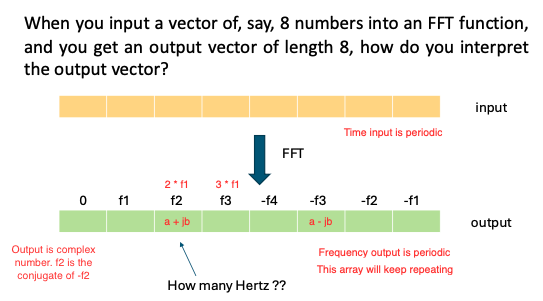
\includegraphics[width=0.95\linewidth]{dft_output.png}
    \item The frequency resolution of the DFT is given by:
    \begin{equation}
      \Delta f = \frac{f_s}{N}
    \end{equation}
    where:
    \begin{itemize}
      \item $f_s$ is the sampling frequency
      \item $N$ is the number of samples
    \end{itemize}
    \item The frequency bins are given by:
    \begin{equation}
      f_k = k \Delta f
    \end{equation}
    \item The DC component (k=0) corresponds to the average value of the signal. It is a constant in the sinusoid equation. The Nyquist frequency (k=N/2) corresponds to the highest frequency that can be represented by the DFT.
    \item We can imagine the DC component as vertical offset of the signal from the x-axis.
    \item \textbf{Visualisation}:
    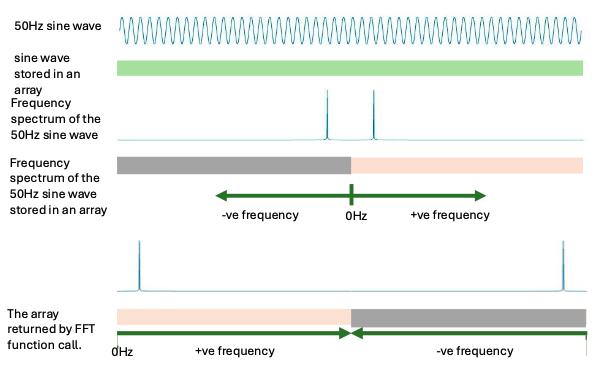
\includegraphics[width=0.95\linewidth]{dft_example.png}
    \item Derivation of the frequency bins:
    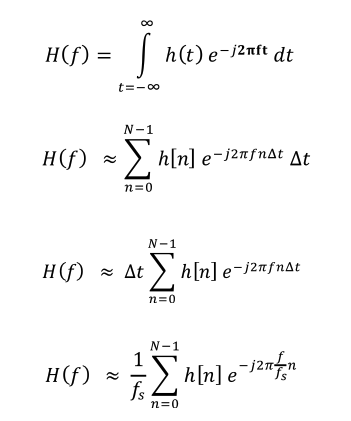
\includegraphics[width=0.55\linewidth, height=120px]{frequency_bin_derivation_1.png}
    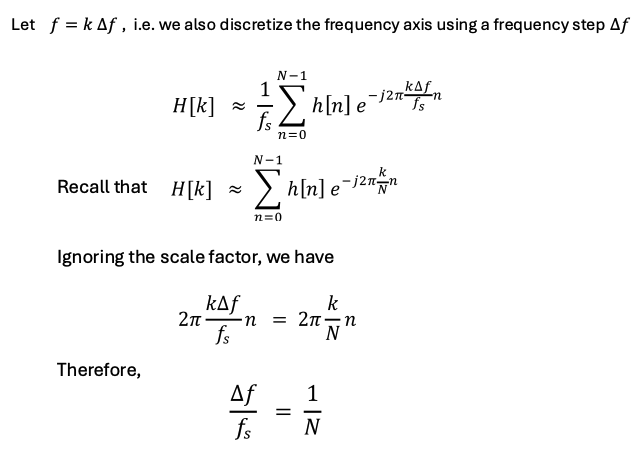
\includegraphics[width=0.95\linewidth]{frequency_bin_derivation_2.png}
    \item \textbf{Note}: Sometimes, we pad the input signal with zeros to increase the number of samples. Padding zeros to the input decreases the frequency bin size, but does not increase the frequency resolution.
    \item \textbf{Note}: N = $2^n$ for FFT, where n is an integer. This is because the FFT algorithm is based on the divide-and-conquer approach, which works best when the number of samples is a power of 2.
  \end{itemize}

  \subsubsection{Properties of DFT}
  \begin{itemize}
    \item \textbf{Intuition}: When you discretise one domain, you also discretise the other domain. The \textit{other domain becomes periodic}.
    \vspace{0.25cm}
    \item \textbf{Linearity}: $\mathcal{F} \{ax[n] + by[n]\} = a X[k] + b Y[k]$
    \item \textbf{Time Shifting}: $\mathcal{F} \{x[n-n_0]\} = X[k] e^{-j 2 \pi k \frac{n_0}{N}}$
    \item If you shift a signal $x[n]$ by $m$ samples in time, the Fourier transform $X[k]$ remains the same in magnitude, but is multiplied by a complex exponential.
    \item This complex exponential introduces a linear phase shift in the frequency domain. This exponential has a magnitude of 1, so the magnitude spectrum stays unchanged.
    \item \textbf{Frequency Shifting}: $\mathcal{F} \{x[n] e^{j 2 \pi m \frac{n}{N}}\} = X[k - m]$
    \item If you multiply $x[n]$ by a complex exponential in the time domain, it causes a circular shift in the frequency domain. Shifting the frequency response by $m$ bins. Both magnitude and phase are affected.
    \item \textbf{Time Reversal}: $\mathcal{F} \{x[-n]\} = X^*[k]$
    \item \textbf{Conjugate Symmetry}: $X[k] = X^*[N-k]$
    \item Here $X^*[k]$ is the complex conjugate of $X[k]$. (i.e If $X[k] = a + jb$, then $X^*[k] = a - jb$)
    \item It is important to note that the $ |X[k]| = |X^*[k]|$
    \vspace{0.25cm}
    \item Conversion \textbf{from continuous to discrete}:
    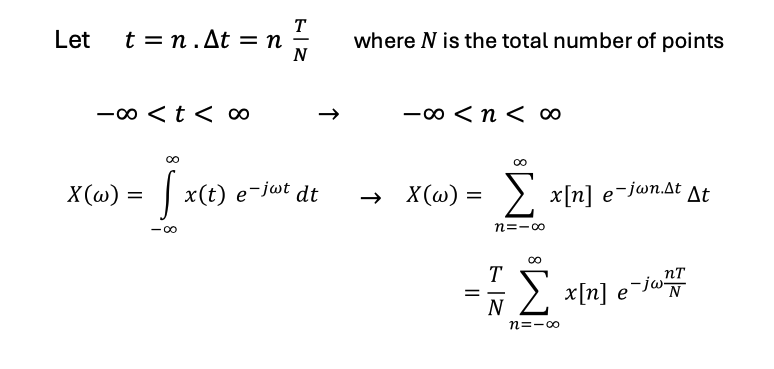
\includegraphics[width=0.95\linewidth]{continuous_to_discrete.png}
    \item \textbf{Note}: $\Delta t = \frac{T}{N}$ \newline
    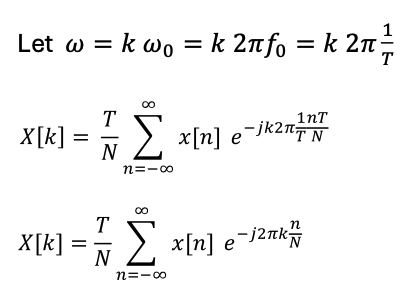
\includegraphics[width=0.55\linewidth]{continuous_to_discrete_2.png}
    \item DFT output is \textbf{periodic with period N} (repeats every N samples). $X[k] = X[k+N]$
    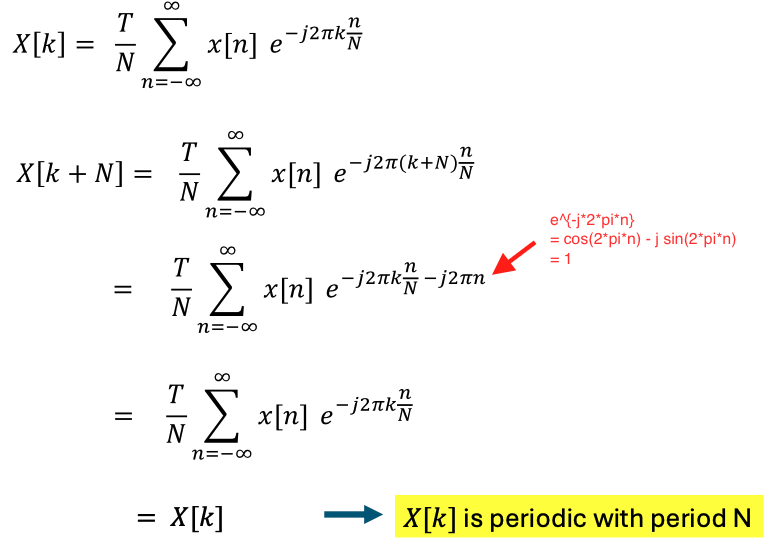
\includegraphics[width=0.95\linewidth]{dft_output_periodicity.png}
    \item Similarly, the input signal is periodic with period N. $x[n] = x[n+N]$
    \begin{equation}
      x[n] = \frac{1}{N} \sum_{k=-\infty}^{\infty} X[k] e^{j 2 \pi k \frac{n}{N}}
    \end{equation}
    \item \textbf{Summary:}
    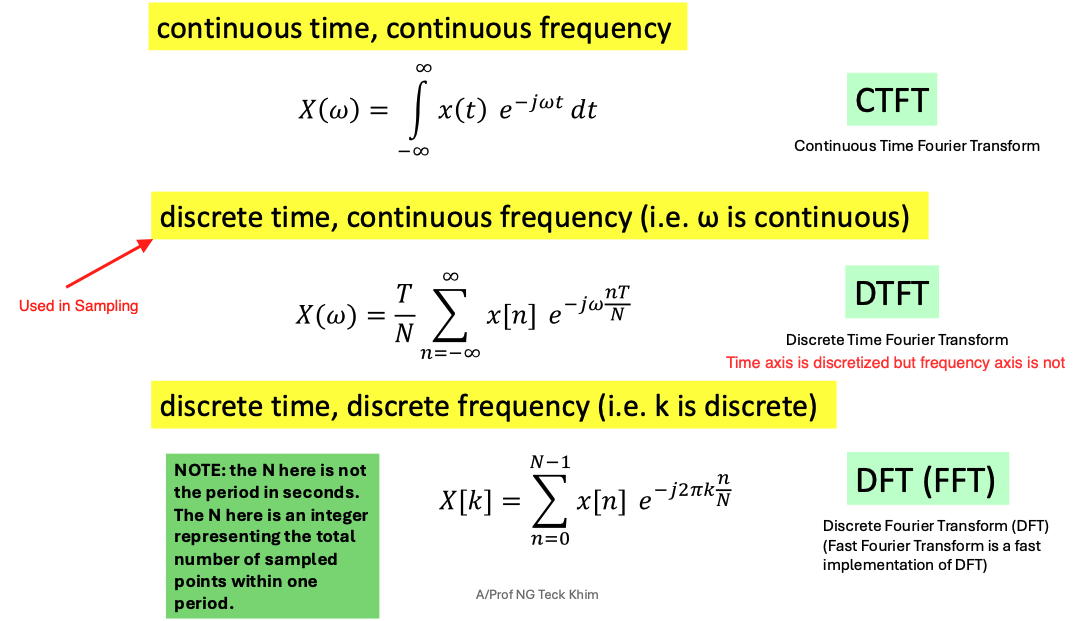
\includegraphics[width=0.95\linewidth]{dft_summary_1.png}
    \vspace{0.15cm}
    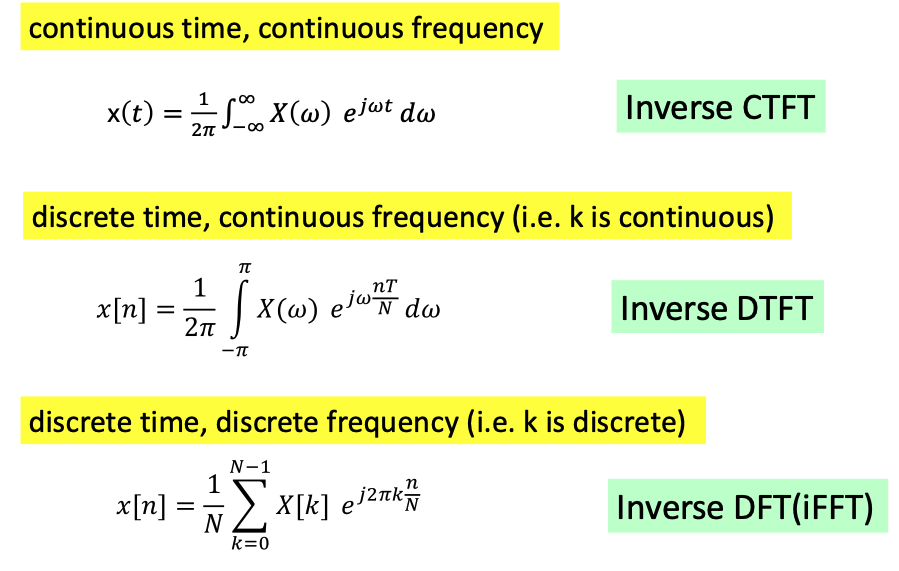
\includegraphics[width=0.95\linewidth]{dft_summary_2.png}
    \vspace{0.15cm}
    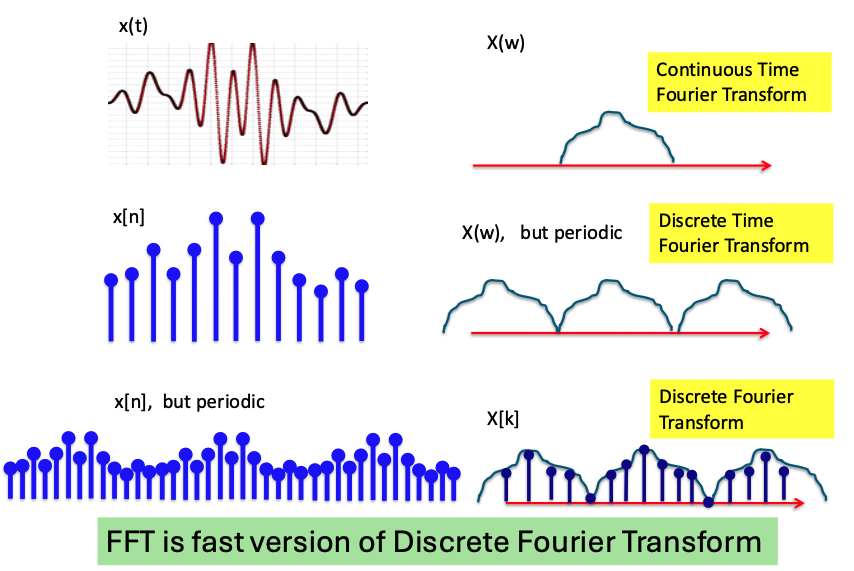
\includegraphics[width=0.95\linewidth]{dft_summary_3.png}
  \end{itemize}
  
  \subsection{Useful Fourier Transform Results}
  \begin{itemize}
    \item Fourier transform of an \textbf{impulse} in the time domain will result in a constant function in the frequency domain. \newline[1, 0, 0, 0] $\rightarrow$ [1, 1, 1, 1]
    \item Fourier transform of a \textbf{constant function} in the time domain will result in an impulse in the frequency domain. \newline[1, 1, 1, 1] $\rightarrow$ [4, 0, 0, 0]
    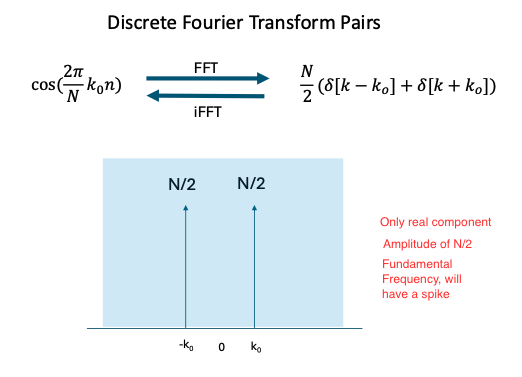
\includegraphics[width=0.95\linewidth]{dft_cosine_pair.png}
    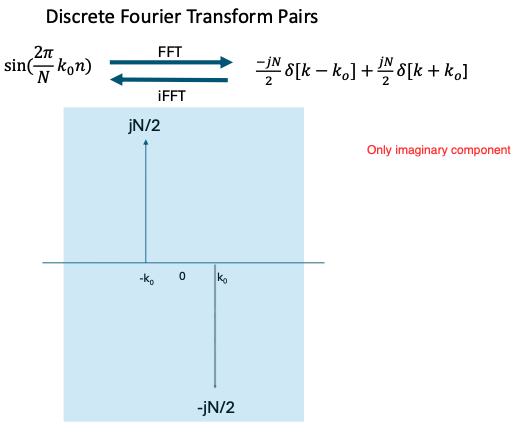
\includegraphics[width=0.95\linewidth]{dft_sine_pair.png}
    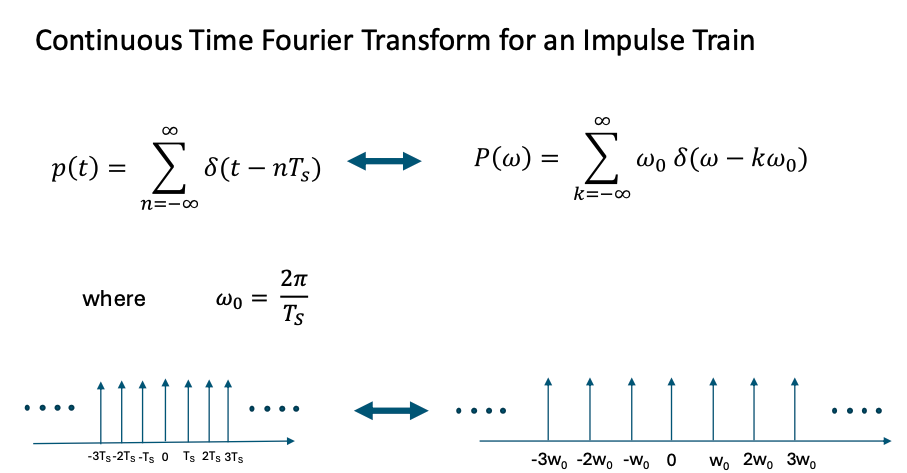
\includegraphics[width=0.95\linewidth]{dft_impulse_train.png}
    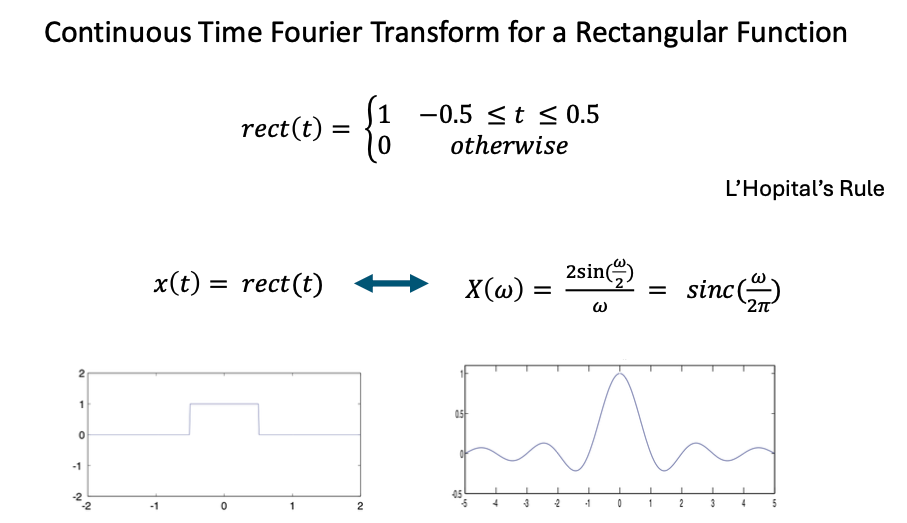
\includegraphics[width=0.95\linewidth]{dft_rect_func.png}
  \end{itemize}

  \section{\underline{2D Fourier Transform}}
  \begin{itemize}
    \item The 2D Fourier transform is used to analyse 2D signals, such as images. Units: \textbf{cycles per meter}.
    \item Sampling frequency: $f_s$ = Number of points/pixels, $N$ per metre
    \item Frequency bin size: $\Delta f = \frac{f_s}{N}$
    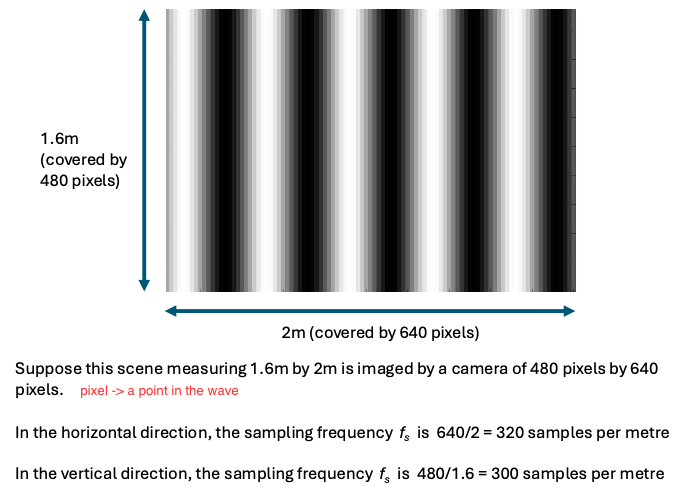
\includegraphics[width=0.95\linewidth]{line_pair_sampling_freq.png}
    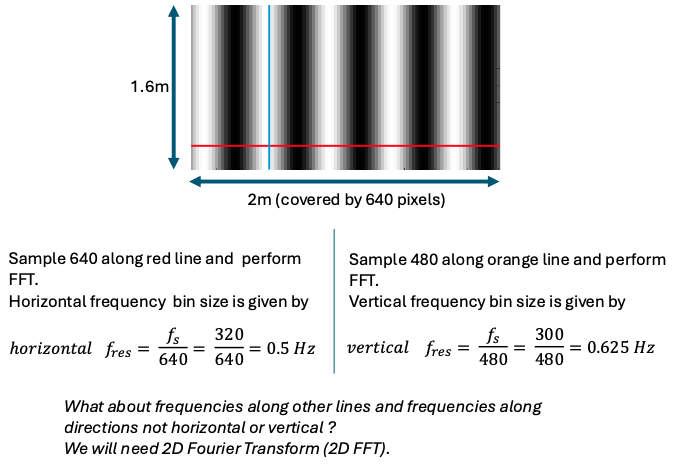
\includegraphics[width=0.95\linewidth]{line_pair_freq_bin_size.png}
    \item \textbf{Intuition:} Applying 1D Fourier transform to each row of the image, then applying 1D Fourier transform to each column of the result.
    \item 2D Fourier transform (spatial domain to frequency domain):
    \begin{equation}
      G[k, l] = \sum_{u=0}^{M-1} \sum_{v=0}^{N-1} g[u, v] e^{-j 2 \pi \left(\frac{ku}{M} + \frac{lv}{N}\right)}
    \end{equation}
    \item 2D inverse Fourier transform (frequency domain to spatial domain):
    \begin{equation}
      g[u, v] = \frac{1}{MN} \sum_{k=0}^{M-1} \sum_{l=0}^{N-1} G[k,l] \cdot e^{j 2 \pi \left(\frac{ku}{M} + \frac{lv}{N}\right)}
    \end{equation}
    where:
    \begin{itemize}
      \item $g[u, v]$ is the input image
      \item $G[k, l]$ is the 2D Fourier transform of the input image
      \item $M$ and $N$ are the dimensions of the image (horizontal and vertical respectively)
      \item $k$ and $l$ are the frequency indices
      \item $u$ and $v$ are the spatial indices
    \end{itemize}
    \item For 2D DFT results with DC component at the top left corner, the top row represents horizontal frequencies, and the left column represents vertical frequencies. 
    \item For 2D DFT results, the output is \textbf{periodic in both dimensions}. The output is a 2D array of complex numbers, where each element represents the amplitude and phase of a specific frequency component in the image.
    \item \textbf{Frequency at peak} = (Coordinate at peak - Coordinate of DC component) $\times$ Frequency bin size
    \end{itemize}

    \section{\underline{Convolution}}
    \begin{itemize}
      \item Convolution is a mathematical operation that combines two functions to produce a third function. 
      \item Convolution is used to filter signals and images. It is used to apply a filter to a signal or image to enhance or suppress certain features.
    \end{itemize}

    \subsection{1D Convolution}
    \begin{itemize}
      \item Process of sliding a window (kernel) over a signal, and computing the weighted sum of the signal values within the window.
      \item The kernel defines the weights, and it is the \textbf{flipped} version of impulse response.
      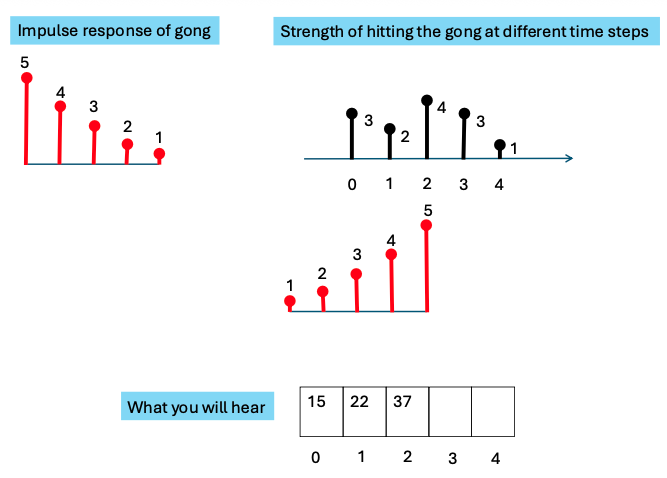
\includegraphics[width=0.95\linewidth]{convolution_impulse_example.png}
      \item Think of the hitting pattern as the signal, and the impulse response as the kernel.
    \end{itemize}

    \subsubsection{Linear Convolution}
    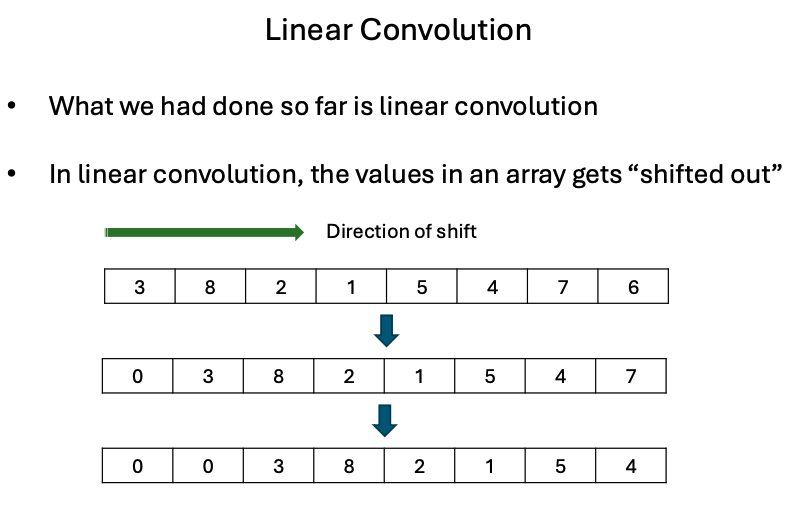
\includegraphics[width=0.95\linewidth]{linear_convolution_array.png}
    \begin{itemize}
      \item Linear convolution can be done in the frequency domain using the Fourier Transform.
      \item \textbf{Linear shift invariance property}: The output of a linear time-invariant system is the convolution of the input signal with the impulse response of the system.
      \item The convolution theorem states that the \textbf{Fourier transform of the convolution of two signals is equal to the product of their Fourier transforms}:
      \begin{equation}
        \mathcal{F} \{x[n] * h[n]\} = X[k] H[k]
      \end{equation}
      \item Derivation of the convolution theorem (discrete version):
      \begin{equation}
        \begin{aligned}
          G[k] &= \mathcal{F}\{g[m]\} = \mathcal{F}\{x[m] * h[m]\} \\
          &= \sum_{m=0}^{M-1} \left( \sum_{\tau=0}^{M-1} x[\tau] h[m - \tau] \right) e^{-j 2 \pi k \frac{m}{M}} \\
          &= \sum_{\tau=0}^{M-1} x[\tau] \left( \sum_{m=0}^{M-1} h[m - \tau] e^{-j 2 \pi k \frac{m}{M}} \right) \\
          &= \sum_{\tau=0}^{M-1} x[\tau] H[k] e^{-j 2 \pi k \frac{\tau}{M}} \\
          &= H[k] \sum_{\tau=0}^{M-1} x[\tau] e^{-j 2 \pi k \frac{\tau}{M}} \\
          &= H[k] X[k]            
        \end{aligned}
      \end{equation}
      \item This uses the circular shift property of DFT, where:
      \begin{equation}
        \mathcal{F} \{h[n-m]\} = H[k] e^{-j 2 \pi k \frac{m}{N}}
      \end{equation}
      \item Note: \begin{tt}{ifft(fft(h(t)) .* fft(x(t)))} \end{tt}
      \item \textbf{Length of the output signal} is $N + M - 1$, where $N$ is the length of the input signal and $M$ is the length of the kernel.
    \end{itemize}

    \subsubsection{Circular Convolution}
    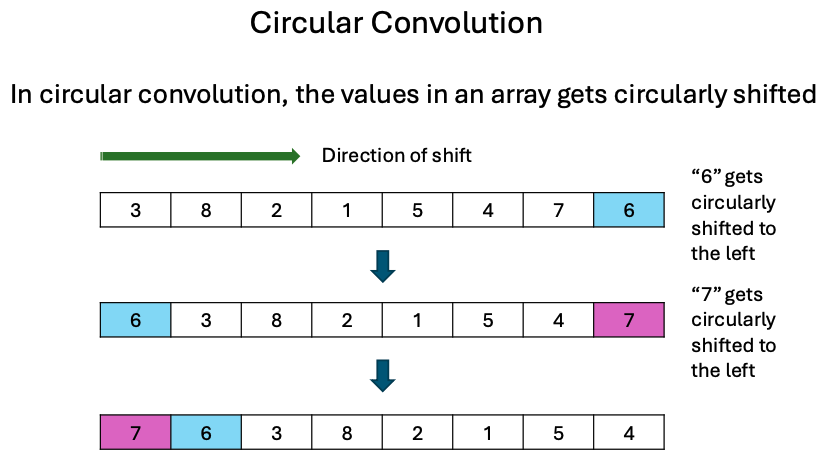
\includegraphics[width=0.95\linewidth]{circular_convolution_array.png}
    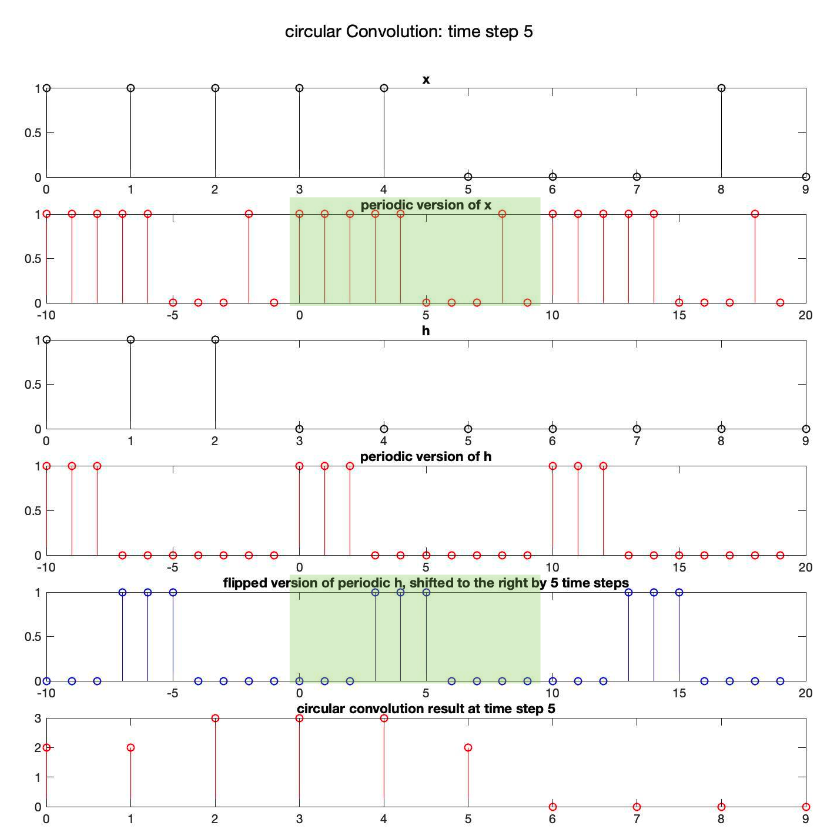
\includegraphics[width=0.95\linewidth]{circular_convolution_example.png}
    \begin{itemize}
      \item Circular convolution is a special case of linear convolution, where the input signal and kernel are both periodic.
      \item To achieve circular convolution, we need to ensure that the input signal and kernel are both periodic with the same period. This is done by \textbf{zero-padding} the input signal and kernel to the same length. 
      \item Normally circular convolution is "unwanted" because it can cause aliasing and distortion in the output signal.
      \item To prevent circular convolution, we can use zero-padding by adding zeros to the input signal and kernel before performing the convolution.
      \item We pad $x[n]$ with $M-1$ zeros, and $h[n]$ with $N-1$ zeros. This ensures that the output signal has a length of $N + M - 1$.
    \end{itemize}

    \subsection{2D Convolution}
    \begin{itemize}
      \item 2D convolution is used to filter images. It is similar to 1D convolution, but it uses a 2D kernel (filter) that slides over the image.
      \item The input image is treated as a 2D array with zeros padded around the edges.
      \item The kernel is flipped in both dimensions before convolution. (left-right and up-down)
      \item The kernel is applied to each pixel in the image, and the output pixel is computed as the weighted sum of the pixels in the kernel.
      \item Start from the top left corner of the image, and slide the kernel over the image.
      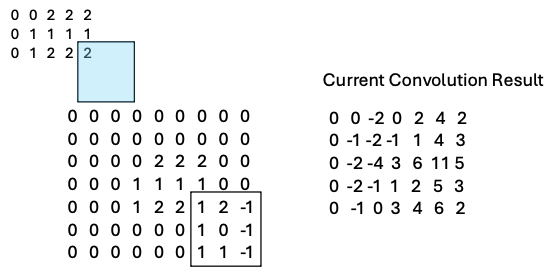
\includegraphics[width=0.95\linewidth]{2d_convolution_example.png}
      \item To implement linear convolution using FFT, we will need to handle the periodicity assumption of the DFT. This is again done by \textbf{zero-padding the input image and kernel}.
      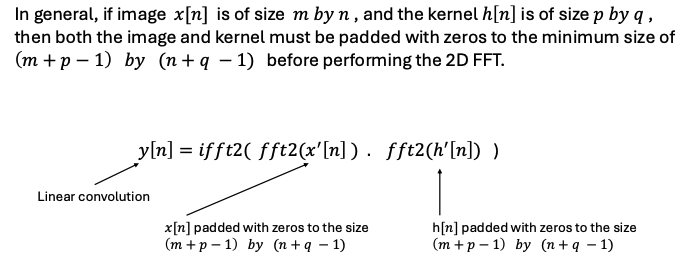
\includegraphics[width=0.95\linewidth]{2d_convolution_zero_padding.png}
      \item For better perforamnce, we can \textbf{pad the input image and kernel to the next power of 2}. This is because the FFT algorithm is based on the divide-and-conquer approach, which works best when the number of samples is a power of 2.
    \end{itemize}

    \section{\underline{Sampling Theorem}}
    \begin{itemize}
      \item Recall that the the Fourier transform of an impulse train is another impulse train.
      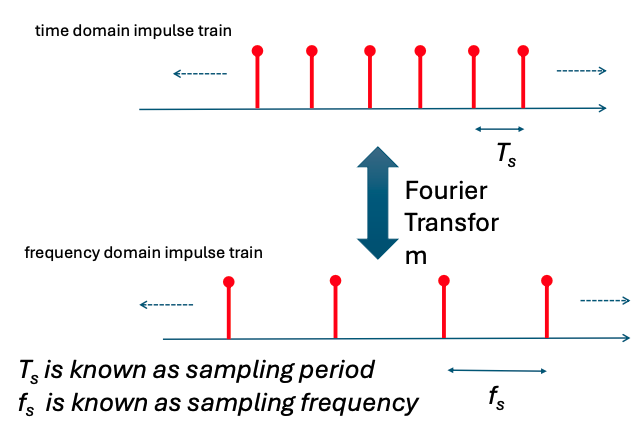
\includegraphics[width=0.95\linewidth]{dft_impulse_train_fs.png}
      \item \textbf{Multiplication in one domain corresponds to convolution in the other domain.}
      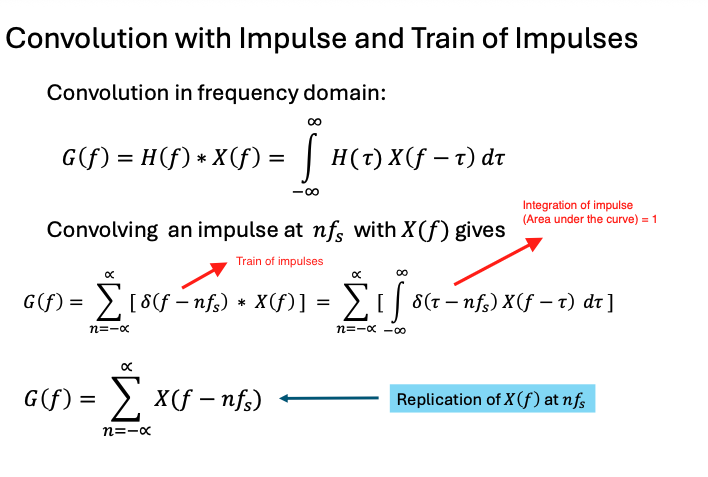
\includegraphics[width=0.95\linewidth]{convolution_train_of_impulses.png}
      \item \textbf{Convolution with a delta function shifts the signal in time.}
      \begin{equation}
        \delta(f - a) * X(f) = X(f - a)
      \end{equation}
      \item Sampling of a signal is represented as multiplcation of the signal (time domain) with an impulse train (time domain).
      \item In the \textbf{frequency domain}, this becomes convolution with an impulse train.
      \item This results in a replication of spectrum $X(f)$ at the integer multiples of the sampling frequency $f_s$.
      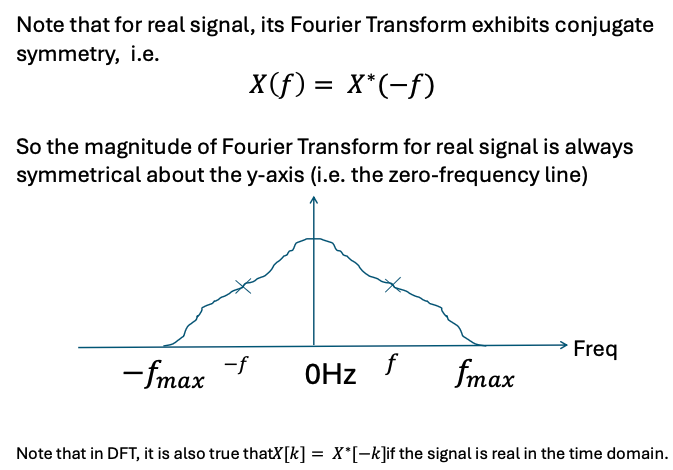
\includegraphics[width=0.95\linewidth]{conjugate_symmetry.png}
      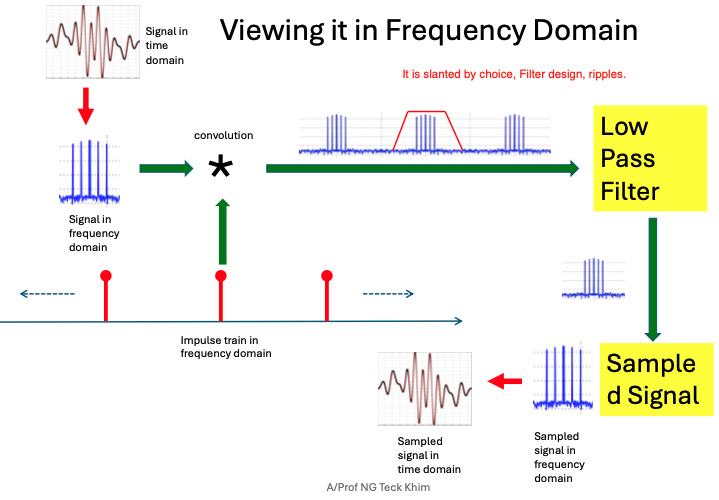
\includegraphics[width=0.95\linewidth]{sampling_frequency_domain.png}
      \item \textbf{Aliasing}:
      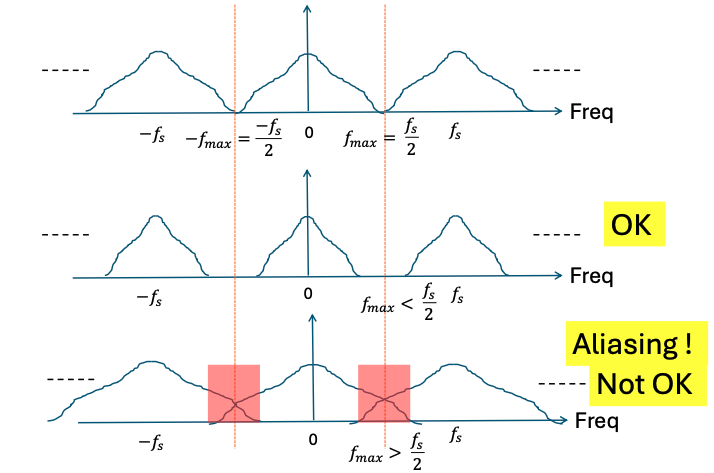
\includegraphics[width=0.95\linewidth]{aliasing.png}
      \item \textbf{Nyquist Rate}: The minimum sampling frequency required to avoid aliasing is twice the highest frequency $f_{max}$ present in the signal.
      \begin{equation}
        f_s > 2 f_{max}
      \end{equation}
      \item Given the maximum sampling frequency available $f_s$, we need to make sure the signal does not contain frequency components above $\frac{1}{2}f_s$.
      \item This can be done by using a \textbf{low-pass filter} before sampling the signal. The low-pass filter will remove the high-frequency components from the signal.
  
    \end{itemize}
    
    \section{\underline{Data Compression}}
    \begin{itemize}
      \item Lossy: JPEG, MP3, MPEG
      \item Lossless: PNG, LZW used in GIF, FLAC
    \end{itemize}

    \subsection{Lossy Compression}
    \begin{itemize}
      \item Sacrifice part of the signal lease critical to human perception.
      \item Image: Missing crispness, color, and detail.
      \item Audio: Missing high pitch sounds, and low volume sounds.
      \item \textbf{Strategy:} Remove high frequency components.
    \end{itemize}

    \subsubsection{Discrete Cosine Transform (DCT)}
    \begin{itemize}
      \item Used in JPEG, MPEG, and MP3 compression.
      \item Similar to Fourier transform, but uses cosine functions instead of sine and cosine functions.
      \item DCT itself is not lossy, it is the filtering of the DCT coefficients that is lossy.
      \item DCT output is real-valued, while DFT output is complex-valued.
      \item \textbf{Recap:} Cosine is an even function, and sine is an odd function. Hence, Fourier transform of cosine is real, and Fourier transform of sine is imaginary.
      \item \textbf{Even function} exhibits symmetry about the y-axis, $x(t) = x(-t)$ \\ \textbf{Odd function} exhibits symmetry about the origin (anti-symmetry) $x(t) = -x(-t)$.
      \item Hence, even signals can be fully represented by cosine functions, and odd signals can be fully represented by sine functions.
      \item Fourier transform of an \textbf{even signal is real} (cosine basis functions only), and Fourier transform of an \textbf{odd signal is imaginary} (sine basis functions only).
      \item There are different types of DCT, but the most common one is \textbf{DCT-II}, which is used in JPEG compression.
      \begin{equation}
        \begin{aligned}
          X[k] & = \sum_{n=0}^{N-1} x[n] \cos\left(\frac{\pi}{N} \left(n + \frac{1}{2}\right) k\right) \\
          & = \sum_{n=0}^{N-1} x[n] \cos\left(\frac{\pi}{N} n k + \frac{\pi}{2N} k\right)
        \end{aligned}
      \end{equation}
      \item \textbf{Intution behind DCT:} Make the signal behave like an even function. Such as flipping the signal about the y-axis, or reverse the signal and add it to the original signal.
      \item We can "downgrade" the high frequency components by:
      \begin{itemize}
        \item \textbf{Zeroing out} the high frequency components in the DCT domain. This is done by setting the DCT coefficients above a certain threshold to zero.
        \item \textbf{Quantization} of the DCT coefficients. This is done by dividing the DCT coefficients by a quantization matrix and rounding the result to the nearest integer. Coarser resolution for high frequency components.
      \end{itemize}
    \end{itemize}

    \subsection{JPEG Compression}
    \textbf{Steps:}
    \begin{itemize}
      \item \textbf{Convert RGB to YCbCr color space}. Y is the luminance (brightness) component, and Cb and Cr are the chrominance (color) components.
      \item Downsample the chrominance components (Cb and Cr) by a factor of 2. This is done because the human eye is less sensitive to color than brightness.
      \item \textbf{Divide the image into 8x8 blocks.}
      \item Apply the \textbf{DCT to each block}. This transforms the image from the spatial domain to the frequency domain.
      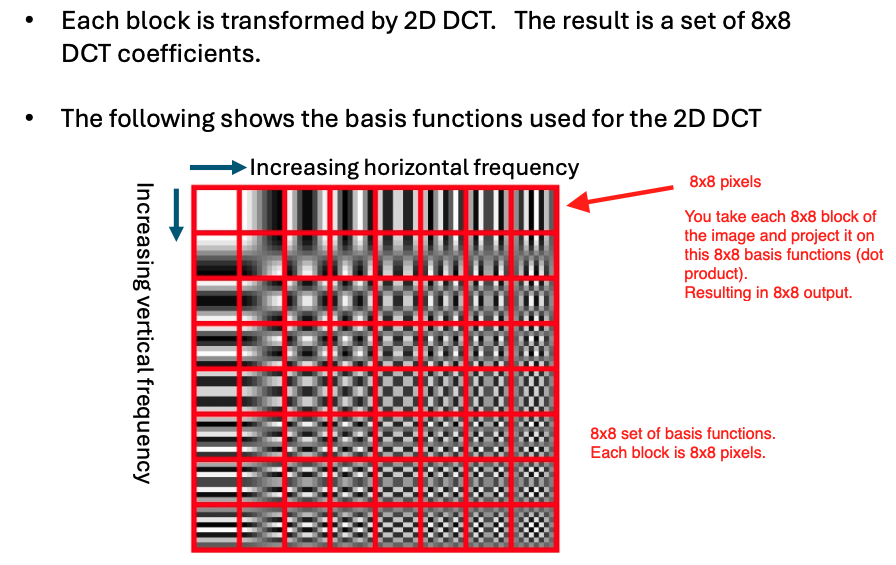
\includegraphics[width=0.95\linewidth]{jpeg_process_1.png}
      \item \textbf{Quantize the DCT coefficients} using a quantization matrix. Higher frequency components are quantized more coarsely than lower frequency components.
      \item Quantization means dividing the DCT coefficients by a quantization matrix and rounding the result to the nearest integer. This reduces the number of bits needed to represent the DCT coefficients.
      \item Luminance channels are quantized with a different matrix than chrominance channels.
      \item Apply \textbf{zig-zag scanning} to the quantized DCT coefficients. This reorders the coefficients in a way that groups the low frequency components together. (So that RLE and Huffman coding can have a higher compression ratio).
      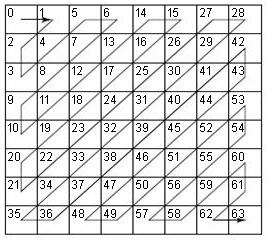
\includegraphics[width=0.55\linewidth, height=100px]{jpeg_zig_zag.png}
      \item Apply \textbf{run-length encoding (RLE)} to the zig-zag scanned coefficients. This compresses the data by replacing consecutive zeros with a single zero and a count of how many zeros there are. (lossless compression)
      \item Apply \textbf{Huffman coding} to the RLE data. (lossless compression)
      \item Store the compressed data in a JPEG file format.
    \end{itemize}

    \subsubsection{Run Length Encoding (RLE)}
    \begin{itemize}
      \item RLE is a simple form of lossless data compression. It replaces consecutive repeated values with a single value and a count of how many times it is repeated.
      \item For example, the sequence [1, 1, 1, 2, 2, 3] would be encoded as [(1, 3), (2, 2), (3, 1)].
      \item RLE is most effective on data with long runs of repeated values. It is not effective on data with high variability.
      \item Another RLE technique is to group consecutive zeros together using a (Run, Value) format:\\
      \textbf{Run} = Number of zeros before a nonzero value.\\
      \textbf{Value} = The next nonzero value.\\
      A special End-of-Block (EOB) marker (e.g., (0,0)) is used to signal the end of nonzero values.
    \end{itemize}

    \subsubsection{Huffman Coding}
    \begin{itemize}
      \item Huffman coding is a \textbf{lossless} data compression algorithm. It replaces frequently occurring values with shorter codes and less frequently occurring values with longer codes.
      \item The algorithm builds a \textbf{binary tree} based on the frequency of each value in the data. The most frequent values are closer to the root of the tree, and the least frequent values are further away.
      \item The code is generated by traversing the tree. A left branch is represented by a 0, and a right branch is represented by a 1.
      \item The resulting binary tree is used to generate \textbf{variable-length codes} for each value in the data. All of which are \textbf{prefix codes}, meaning no code is a prefix of another code.
      \item \textbf{Algorithm:}
      \begin{itemize}
        \item Create a min-heap (priority queue) where each node is a character and its frequency.
        \item While more than one node in the heap:
        \begin{itemize}
          \item Renive the two nodes with the lowest frequency.
          \item Create a new internal node with these two as children
          \item The new nodes frequency is the sum of the frequencies of its children.
          \item Insert the new node back into the heap.
        \end{itemize}
        \item The remaining node is the root of the Huffman tree.
      \end{itemize}
      \item With Huffman coding, we need to \textbf{send the Huffman tree} along for decoding.
      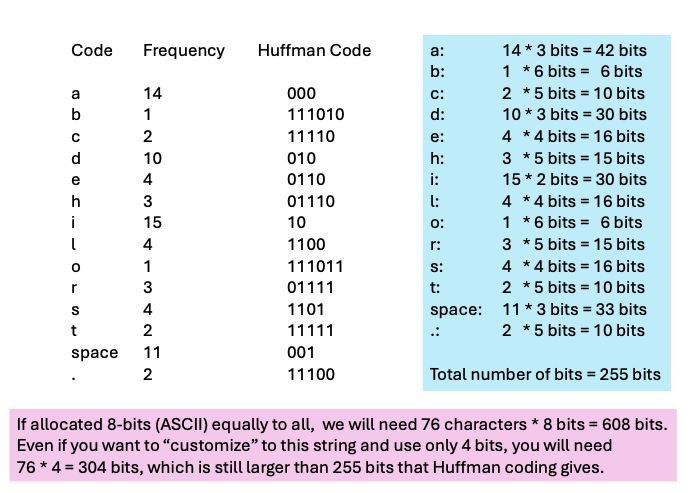
\includegraphics[width=0.95\linewidth]{huffman_coding.png}
    \end{itemize}
    
    \subsection{Lempels-Ziv-Welch (LZW) Compression}
    \begin{itemize}
      \item LZW is a \textbf{lossless} data compression algorithm. It replaces repeated sequences of data with a single code.
      \item Used in GIF and TIFF image formats, Unix file compression utility compress.
      \item \textbf{Encodes 8 bit data using n bit codes}, where $n > 8$. 0-255 are the original 8 bit data, and 256-4095 are the new codes and data dependent.
      \item The algorithm starts with a dictionary of all possible single-character sequences. As it processes the data, it adds new sequences to the dictionary.
      \item When it encounters a sequence that is already in the dictionary, it replaces it with the corresponding code.
      \item We don't need to send the dictionary along with the compressed data, because the decoder can build the same dictionary from the compressed data.
      \item \textbf{Encoding Algorithm:}
      \begin{itemize}
        \item Initialize the dictionary with all possible single-character sequences.
        \begin{itemize}
          \item Read the longest sequence W found in the dictionary.
          \item Output its corresponding code.
          \item Read the next character K.
          \item Add W + K to the dictionary with the next available code.
          \item Repeat until the end of the data.
        \end{itemize}
      \end{itemize}
      \item \textbf{Decoding Algorithm:}
      \begin{itemize}
        \item Initialize the dictionary with all possible single-character sequences.
        \item Read the first code and output the corresponding sequence.
        \item Set this sequence as the \texttt{previous sequence}.
        \item \textbf{While} there are more codes:
        \begin{itemize}
          \item Read the next code.
          \item \textbf{If} the code exists in the dictionary:
          \begin{itemize}
            \item Let \texttt{entry} be the corresponding sequence.
          \end{itemize}
          \item \textbf{Else} (edge case: code not in dictionary yet):
          \begin{itemize}
            \item Let \texttt{entry} = \texttt{previous sequence + first character of previous sequence}.
          \end{itemize}
          \item Output \texttt{entry}.
          \item Add \texttt{previous sequence + first character of entry} to the dictionary.
          \item Set \texttt{previous sequence = entry}.
          \end{itemize}
       \end{itemize}
       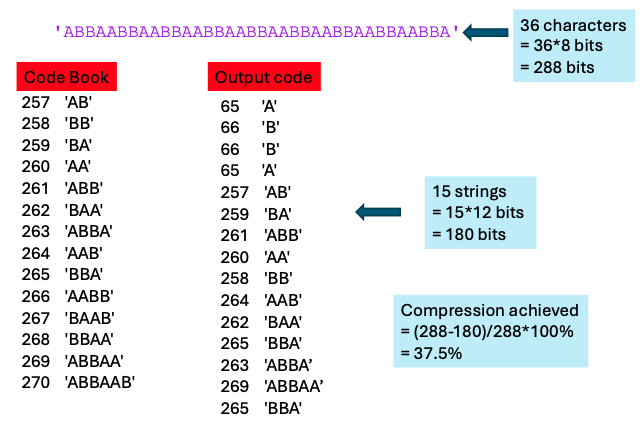
\includegraphics[width=0.95\linewidth]{lzw_result_example.png}
       \item Because we set it to $4096 = 2^{12}$ entries, we can use 12 bits to represent the codes. Although in this case, 9 bits would have sufficed as 270 codes were used.
      \end{itemize}
\end{multicols*}

\end{document}
